\begin{Exercise}[label = carts, origin = {III. IPhO, Tschechoslovakei}, title = Boxen,difficulty = 3]
	Die drei Boxen $A$, $B$ und $C$ sind wie in Abb. \ref{fig:cartss} gezeigt positioniert. 	
\end{Exercise}
\begin{figure}[h]
	\centering
	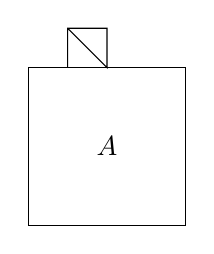
\begin{tikzpicture}
		\draw(-2,0)--(-2,2)--(0,2)--(0,0)--(-2,0);
		\node at (-1,1) {$A$};
		\draw(-1.5,2)--(-1.5,2.5)--(-1,2.5)--(-1,2)--(-1.5,2.5);
	\end{tikzpicture}
	\caption{Anordnung}
	\label{fig:cartss}
\end{figure}